\documentclass{article}
\usepackage[utf8]{inputenc}

\usepackage{geometry}
 \geometry{
 a4paper,
 %total={170mm,257mm},
 left=15mm,
 top=15mm,
 right=15mm,
 bottom=25mm,
 }
 
\usepackage{graphicx}
\graphicspath{ {./img} }
\usepackage{caption}
\newenvironment{Figure}
  {\par\medskip\noindent\minipage{\linewidth}}
  {\endminipage\par\medskip}
 
\usepackage{hyperref}
\hypersetup{
    colorlinks=true,
    linkcolor=blue,
    filecolor=magenta,      
    urlcolor=blue,
}
 
\usepackage{amsmath}
 
% Checkmark symbol
\usepackage{amssymb}
% Crossmark symbol
\newcommand{\xmark}{\times}

\usepackage{multicol}


\newenvironment{myitemize}
{ \begin{itemize}
    \setlength{\itemsep}{005pt}
    \setlength{\parskip}{0pt}
    \setlength{\parsep}{0pt}     }
{ \end{itemize}                  } 

\title{EPFL Computer Security Summary}
\author{Matthias Zeller}
\date{June 2020}

\begin{document}

\maketitle

\begin{multicols}{2}
\tableofcontents
\newpage


% ========================================================================

\section{Access control}

= determining whether a principal has authorized access to an object. An authorization is a tuple (principal, access, object).

\paragraph{Terminology}

\begin{myitemize}
    \item \textbf{Subjects} (often = principal) = entity within an IT system
    \item \textbf{Object} (=asset) = resources that subject may access or use
    \item \textbf{Operation} = read, write, append, execute
\end{myitemize}

\subsection{Access Control Matrix (ACM)}

\begin{myitemize}
    \item Abstract representation of all permitted triplets (subject, action, access right)
    \item Must be dynamic
    \item 2nd role: determine which subjects can provide permissions on objects to other subjects
    \item Must implement security policy without ever violating it
    \item Not suitable for direct implementation
    \begin{myitemize}
        \item Not scalable
        \item Very sparse $\rightarrow$ inefficient
        \item Error prone: no global view
    \end{myitemize}
\end{myitemize}

\paragraph{Graham-Denning Model}

Extends matrix with:

\begin{myitemize}
    \item Ownership: each object has owner = subject that creates the object
    \item Controllership: each subject has a controller = subject that creates the subject
    \item Allows delegation and revocation
\end{myitemize}

\subsection{Types of access control}

\begin{myitemize}
    \item \textbf{Mandatory access control} (MAC): central authority (military, hospital, baking)
    \item \textbf{Discretionary access control} (DAC): object owner assign permissions
\end{myitemize}

\subsection{How to store an ACM}

\subsubsection{Access Control List (ACL)}

\begin{myitemize}
    \item Store the access control matrix by column
    \item Permissions are associated to \textbf{objects}
    \item Stored with the resource
    \item Easy to determine who can access a resources
    \item Difficult to see all rights of a user
    \item Difficult permission delegation
    \item Difficult to check at run-time, confused deputy problem, not always clear which subject accesses the resource
    \item Unsuited for systems with many subjects that come and go $\rightarrow$ large dynamic ACL, two alternatives:
    \begin{myitemize}
        \item Role-based access control
        \item Group-based access control
    \end{myitemize}
\end{myitemize}


\subsubsection{Capability}

\begin{myitemize}
    \item Store ACM by row
    \item Permissions associated to subjects
    \item Stored with the subjects
    \item Easy to visualize all subject permissions
    \item Easy to delegate
    \item Revoking permissions on one object is hard
    \item Hard to ensure legitimate access right transfer
\end{myitemize}


\subsection{Role-based access control (RBAC)}

\begin{myitemize}
    \item Assign permissions to roles, assign roles to subjects, subjects select an active role
    \item Rationale: some subjects are similar to each other and have the same rights
    \item Alternative to ACLs systems having many subjects that come and go
    \item Problems:
    \begin{myitemize}
        \item Role explosion, temptation to fine grain roles
        \item Limited expressiveness: problem with least privilege
        \item Difficult to implement separation of duty, pb with separation of privilege 
    \end{myitemize}

\end{myitemize}

\subsection{Group-based access control}

\begin{myitemize}
    \item Assign permissions to access objects to groups, assign subjects to groups, subjects have the permission of all their group
    \item Rationale: some permissions are always needed together (e.g. access to sockets and access to network interface)
    \item Alternative to ACLs systems having many subjects that come and go
    \item Supports negative permissions, they’re always tested first 
\end{myitemize}


\subsection{Example: UNIX/Linux access control}

\begin{myitemize}
    \item Principals and groups:
    \begin{myitemize}
        \item User (= principal) identities UIDs, group identities GIDs
        \item User information
        \item Users belong to >= 1 group
    \end{myitemize}

    \item Security architecture
    \begin{myitemize}
        \item Discretionary access control
        \item Each user owns a set of files 
        \item All processes of a user run with that user’s privileges = ambient authority
        \item 3 “groups”: owner, group, other
    \end{myitemize}

    \item Super users
    \begin{myitemize}
        \item Special root user account
        \item Can access everything, no access deny
        \item Almost no security checks
        \item Root is in the Trusted Computer Base (TCB)
    \end{myitemize}

    \item Access control Lists
    \begin{myitemize}
        \item Files have ACLs attached: each file has a owner UID and GID assigned, 9 permission bits
        \item Different semantics between files and directories
        \item 3 attributes: suid, sgid, sticky
    \end{myitemize}

    \item Access control implementation:
    \item Special rights: suid, sgid
\end{myitemize}

\subsection{Ambient authority}

\begin{myitemize}
    \item Implicit subject and authority, only operation and names are specified
    \item Simplifies program design and usability
    \item Problem with least privilege 
    \item ACL generally considers ambient authority, permissions usually checked for the user running the program
    \item Capabilities: they themselves contain the identity of the principal, no ambient authority
    \item \textbf{Confused deputy}: privileged principal used by another less privileged principal to improve its access. To avoid those problems:
    \begin{myitemize}
        \item Re-implement access control in the privileged process: expensive, cumbersome, error-prone
        \item Let privileged process check authorizations 
        \item Use capabilities instead of ACLs
    \end{myitemize}
\end{myitemize}


\subsection{Access contorl implementation}

Should use reference monitor: check everything. Do NOT check accesses all over the program. This violates the least common mechanism principle. This supports economy of mechanism and complete mediation. 


% ==================================================================

\section{Security models}

For instance, when considering the type of access control (MAC, DAC), we can wonder about the basic security principles behind these policies. We can ask: "Are there things owners of objects are \emph{not} allowed to do ?". Yes $\rightarrow$ MAC, no $\rightarrow$ DAC. 

The lecture focuses on the MAC security policy models. These policies determine all relations between subjects and objects. The user and owner of an object has no rights to establish access policy of the object. 

\subsection{What are Security Models?}

\begin{myitemize}
    \item Not a policy or mechanism itself
    \item Design pattern to reason about security properties to build security policies
    \item Doesn't provide details of the policy
    \item A security model might or might not be appropriate for a specific security property
    \item First security model: Orange Book, covers (mainly) needs of government for confidentiality 
\end{myitemize}

\subsection{The Bell-LaPadula Model (BLP)}

\begin{myitemize}
    \item \textbf{Multilevel} security approach
    \item Tackle the \textbf{confidentiality} problem
    \item Family of models subject to refinement and extensions
\end{myitemize}

\subsubsection{Overview on BLP Components}

\begin{myitemize}
    \item Subjects S and Objects O
    \item Access to objects: 4 values, execute, read, write, append (i.e. can't read, only add content at the end)
    \item System state
    \begin{myitemize}
        \item Level functions: mapping subject/objects to classifications
        \item Access Control Matrix
        \item Current access set: current authorized triplets in the system (subject, object, attribute)
    \end{myitemize}
\end{myitemize}

\subsubsection{Level function for objects: Classification}

\begin{myitemize}
    \item Classification: total order of labels (\textit{e.g. Unclassified, Confidential, Secret, Top Secret})
    \item Categories: compartments of objects on one topic (\textit{e.g. Nuclear, Crypto})
    \item Security level = (Classification, \{set of categories\})
\end{myitemize}

\paragraph{Dominance relationship}

\begin{myitemize}
    \item Dominance relationship: level (l1, c1) dominates level (l2, c2) if:
    \begin{myitemize}
        \item l1 $\geq$ l2 ($\geq$ means more secret than)
        \item c2 $\subset$ c1
    \end{myitemize}
    \item Representation: Lattice
    \item Properties: dominance is transitive, top and bottom levels, no total order (\textit{i.e. some have no relationship})
\end{myitemize}

\paragraph{Clearance level}

\begin{myitemize}
    \item Clearance = maximum security level a subject has been assigned
    \item Current security level: subjects can operate at lower security levels
    \item $\text{level}(S_i)$ must dominate $\text{current\_level}(S_i)$
\end{myitemize}

\subsubsection{BLP properties}

\paragraph{Simple security property}

\begin{myitemize}
    \item SS-property: if (subject, object, w/r) is a current access, then level(subject) dominates level(object)
    \item In other words, a subejct can read objects with lower classification than its clearance
    \item Also called No Read Up (NRU)
    \item Not sufficient though: just forbidding people to read up doesn't prevent malicious code to high level classified information to lower levels (violates the ss-property)
\end{myitemize}

\paragraph{Star property}

\begin{myitemize}
    \item *-property: if subject has simulatneous observe (r,w) access to $O_1$ and alter (a,w) access to $O_2$, then level $O_2$ dominates $O_1$
    \item In other words, a subject cannot  write in clearance levels lowers than theirs, so they cannot leak information
    \item Due to ss-property (no read up), the subject can only append to higher levels
\end{myitemize}

\paragraph{Discretionary property}

\begin{myitemize}
    \item ds-property: if an access (subject, object, action) takes place it must be in the access control matrix
    \item Information should only be accessed on a need-to-know basis $\rightarrow$ least privilege principle
    \item Using DAC, the system can protect integrity of objects by forbidding subjects from writing
    \item This is basically saying that we use an ACM
\end{myitemize}

\subsubsection{Basic Security Theorem}

\begin{myitemize}
    \item If all state transitions are secure, and the initial state is secure, then every subsequent state is secure regardless of the inputs
    \item If for any individual access, the ss-property, the *-property and the ds-property hold, then any sequential composition security holds
    \item $\Rightarrow$ a system can be analyzed in terms of single step transitions of state
    \item Remind: a state is the current access permissions, the ACM and the clearance level
\end{myitemize}

\subsubsection{BLP Problems}

\begin{myitemize}
    \item Confidentiality-oriented: does not consider integrity or availability
    \item State-based + single transition model: too low-level, not expressive
    \item the 3 security properties are not sufficient to ensure confidentiality
\end{myitemize}


\paragraph{Illegal information flow}

If level($S_1$) is TS (Top Secret), level($S_2$) is C (Confidential):

\begin{enumerate}
    \item $S_2$ creates $O_2$ $\rightarrow$ level($O_2$) = TS
    \item $S_1$ reads C and either:
    \begin{myitemize}
        \item changes the object level
        \item leaves object level untouched 
    \end{myitemize}
    \item $S_2$ attempts to access to $O_2$ in C $\rightarrow$ success or failure leaks 1 bit of information
\end{enumerate}


\subsection{Covert channels}

\begin{myitemize}
    \item Covert channel: any channel that allows information flows contrary to the security policy
    \item A covert channel is enabled by shared resources accessed by subjects with different clearance levels
    \item Least common mechanism: the more resources are shared, the harder it is to eliminate covert channels 
    \item Eliminate covert channels: 
    \begin{myitemize}
        \item Isolate the high level: once information is up don't let it go down. But not practical
        \item Add noise to communications: add fake interaction between high and low levels such that real intended covert channels cannot be distinguished from random noise
        \item With 1 bit/second of leak, OK for documents, not ok for cryptographic keys
        \item DoD policy: store cryptographic keys on dedicated hardware
    \end{myitemize}
\end{myitemize}

\subsubsection{The tranquillity property}

\begin{myitemize}
    \item Tranquillity: classification/clearance does not change during execution
    \item Illegal flows are enabled by actions in the system not rules by the BLP rules: changes in object/subject levels,  changes in the ACM
    \item But static is not practical
\end{myitemize}


\subsection{Declassification}

\begin{myitemize}
    \item With no write down, how a subject communicates with lower level subjects ?
    \item Declassification: remove classification label, under the control of the security policy
    \item Enables communication with lower layers
    \item Cannot be made inherently safe, manual process
    \item Very typical and necessary
    \item Hard to rule out covert channels (how to know the object does not contain secrets?)
\end{myitemize}


\paragraph{Difficulty of declassification in practice}

\begin{myitemize}
    \item Microsoft Word revision history contains deleted text
    \item PDF redaction by overlying graphical elements, the text is on the file!
    \item Strategic adversary!
\end{myitemize}

\subsection{NRL pump}

\begin{myitemize}
    \item System that implements BLP by inserting a router that physically separates communications between high and low levels 
    \item High can read low, but can't write low
    \item There is a covert channel: acknowledgments. 
    \begin{myitemize}
        \item Low levels need ACKs from high levels to know if information is delivered
        \item These ACKs could be used as covert channels (e.g. by introducing delays)
        \item Avoid problem: the pump buffers the ACK and delivers it after a probabilistically based time (???)
    \end{myitemize}
    
\end{myitemize}


\subsection{Integrity}

\begin{myitemize}
    \item Integrity also matters! 
    \item Preventing fraud (e.g. in commercial services) is about protecting integrity
    \item Public key cryptography requires high-integrity for confidentiality
    \item Properties of integrity: for (a,b) inputs of an operation yielding a result, the adversary cannot
    \begin{myitemize}
        \item influence inputs from honest parties
        \item exchange the operation for another one
        \item change the result
        \item perform the operation more than once
    \end{myitemize}
    \item The system should operate as if no adversary tries to tamper with it
\end{myitemize}

\subsubsection{Principles of Integrity mechanisms}

\paragraph{Separation of duties}

Require multiple principals to perform an operation (separation of privilege principle). Examples: accountant records payments/income (the two must match), both sides of a transaction keep a record and must match (legal receipts), two officers requires to launch a missile.

\paragraph{Rotation of duties} 

Allow a principal only a limited times on a particular role \& limit other actions while in this role. This decreases opportunities of principals to tamper with the action. Examples: guards appointed for a single random shift to guard a bank safe. 

\paragraph{Secure logging}

Tamper evident log to recover from integrity failures (compromise recording principle). Consistency of log across multiple entities is the key. Needs separation and rotation of duties principle. Examples: logs of transactions inside ATM machine, notaries maintain logs of transactions and contracts, bitcoin. 


\subsection{The BIBA Model}

\begin{myitemize}
    \item Multilayer security approach
    \item Tackles the \textbf{integrity} problem
    \item Family of models subject to refinement and extensions
    \item Subjects and objects are assigned an integrity level
    \item Two strict key rules
    \item Simple integrity: \textbf{no read-down}, protect higher integrity principals from being corrupted by lower integrity level data
    \item *-integrity: \textbf{no write-up}, prevent lower integrity principals from being corrupting high integrity data
    \item Examples: in bank, director establishes rules and every employee reads, employees cannot rewrite rules. Computer: Web application open in the browser should not write to the file system (at most /tmp)
\end{myitemize}


\subsubsection{BIBA variant : Low-water-mark for subjects}

\begin{myitemize}
    \item Low-water-mark policy for subjects: subjects start processes at their highest integrity level. When accessing an object, its current level is lowered to the lowest of the two: current-level(s), level(o)
    \item Temporary downgrade for the session: hard to avoid label creep. Example: mitigate impact of a network Trojan. 
\end{myitemize}

\subsubsection{BIBA variant 2: Low-water-mark for object}

\begin{myitemize}
    \item Low-water-mark for objects: once object has been written by a subject, it takes the lowest level of the object or subject
    \item Dangerous! Only allows for integrity violation detection, the file cannot harm but tampering has happened
    \item Idea: if subject pollutes an object by writing on it, this object is downgraded to the level of the subject
    \item Option to prevent tampering: replicate, and once operation happended, either sanitize or upgrade
\end{myitemize}

\subsubsection{BIBA Additional actions}

\paragraph{Invocation}

\begin{myitemize}
    \item Subjects can interact with objects at other levels, but still protecting the object
    \item For instance, a Director acts as a protection (run checks or deny operations) for the object that the Teller needs to write on. 
    \item Simple invocation: high level invoke low level $\rightarrow$ protects high level data. Problem: unclear who modified an object
    \item Controlled invocation: low level invoke high level $\rightarrow$ prevent corruption of high integrity data. Problem: hard to check that no secret is actually written in high integrity objects
\end{myitemize}

\subsubsection{Sanitization}

\begin{myitemize}
    \item Sanitization: process of taking objects with low integrity and lifting them to high integrity
    \item Root cause of large classes of real-word security vulnerabilities: low input (user) can influence high data and code (service)
    \item Example: Web server (high) accepts input from web client (low) $\rightarrow$ SQL injection. 
\end{myitemize}

\paragraph{Fail-safe default}

\begin{myitemize}
    \item Positively verify that low objects are within a valid set before elevating their integrity to high
    \item White list: check that all properties of good objects hold
    \item Do NOT blacklist: or at least, not only 
\end{myitemize}


\subsection{Combining security properties}

\begin{myitemize}
    \item Secure composition of mechanisms is hard! 
    \item Composing confidentiality and integrity:
    \begin{myitemize}
        \item BLP: confidentiality, no integrity
        \item BIBA: integrity, no confidentiality
        \item Chinese Wall Model
    \end{myitemize}
    \item From multi-level to mutli-lateral security
    \begin{myitemize}
        \item Different entitites seek for different propertiesvu croix englais
        \item Properties may have conflicting requirements
        \item Who secures the TCB? 3rd party (pb: trust), trusted hardware (pb: trust manufacturer), advanced cryptography 
    \end{myitemize}
\end{myitemize}


\subsubsection{Chinese Wall Model}

\begin{myitemize}
    \item Inspiration: UK rules about handling conflicts of interest in the financial sector
    \item All objects associated with label denoting their origin (e.g. Coca-cola, Pepsi)
    \item Originators define conflict sets of labels (e.g. Pepsi and Coca-cola is a set)
    \item Subjects are associated with a history of their accesses to objects and their labels

\end{myitemize}

\paragraph{Access rules}

\begin{myitemize}
    \item Direct flow: a subject can read/write and object if the access does not allow an information flow between items in the same conflict set
    \item Indirect flow: access denied. Happens when A works in Pepsi, B in Coca-Cola, and A and B meet in IBM. 
    \item Enable flexibility (which is restricted due to indirect flow): must sanitize: un-label some items as long as information cannot lead to conflicts of interest. Indirect flow 
\end{myitemize}


% ======================================================0

\section{Applied cryptography}

Example of an everyday declassification act: publishing code on Github. Many developpers are unknowingly posting their hardcoded credentials online. See the \href{https://github.com/zricethezav/gitleaks}{gitleaks} repository which uses regexp and entropy (cool!). 

\subsection{Why Cryptography Matters?}

\begin{myitemize}
    \item Frees you from physical security
    \item Reduces the TCB to the confidentiality and integrity of the keys
    \item We don't always a TCB (e.g. while data is in transit), so cryptography is useful in this case
\end{myitemize}

\subsection{Terminology}

\begin{myitemize}
    \item Confidentiality: unauthorized parties cannot access information
    \item Plaintext: non-encrypted message, readable
    \item Cryptographic algorithm: set of mathematical instructions to encrypt and decrypt data
    \item Ciphertext: encrypted message obtained by using cryptographic algorithm and plaintext
    \item Unlike encoding, encryption and decryption require a key
    \item Cryptographic primitives: universal, exchangeable cryptographic building blocks. Either can't break it down any further or no security argument for its individual parts
\end{myitemize}

\subsection{History - Quest for confidentiality}

\begin{myitemize}
    \item Ceasar's cipher (50 BC) and Kamasutra cipher (400 AD) can be very easily broken with frequency analysis
\end{myitemize}

\subsection{One Time Pad}

\begin{myitemize}
    \item Key = string of random bits as long as the message 
    \item Prevents frequency analysis (repeated characters are encrypted to different values)
    \item Must never reuse OTP key: even if cannot recover full message, can recover information for frequency analysis 
    \item Problems: key as long as message, key must be random, key cannot be reused, no integrity
\end{myitemize}

\subsection{Symetric encryption}

\begin{myitemize}
    \item Same key for encryption and decryption
    \item Two types of cipher: block and stream ciphers
    \item Integrity mechanism: MAC
\end{myitemize}

\subsubsection{Stream cipher}

\begin{myitemize}
    \item Key: small
    \item Initialization vector: not secret, must not be reused. Purpose: same messages encrypted with the same key are different. 
    \item Stream ciphers output stream of bits that is pseudorandom 
    \item Security argument: pseudo-randomness of stream
    \item Remaining downsides (w.r.t. OTP): key must be random, no integrity
    \item Strengths: fast and low error propagation
    \item Weaknesses: Low diffusion (all information of a plaintext symbol contained in one ciphertext symbol) and susceptibility to insertions/modifications (difficult to detect)
\end{myitemize}

\subsubsection{Block ciphers}

\begin{myitemize}
    \item Key = short random string of fixed size
    \item Encrypts blocks of short key-size
    \item Messages often > 1 block, need to chain blocks together with \textbf{modes of operation}:
    \begin{myitemize}
        \item Electronic code book (ECB): independent blocks, don't use, $m_1=m_2 \Rightarrow c_1=c_2$
        \item Cipher block chaining: encryption depends on previous blocks, need an IV each time. Problem: if IV is wrong (but known key), only the first block is corrupted
        \item Counter mode (CTR): turns the block cipher into stream cipher, need a nonce, encryption same as decryption
    \end{myitemize}
    \item Stengths: high diffusion, easy tampering detection
    \item Weaknesses: slow (must accumulate an entire block before encryption/decryption), error propagation (depends on mode of operation)
\end{myitemize}


\subsection{Integrity (symmetric)}

\subsubsection{Message Authentication Code (MAC)}

\begin{myitemize}
    \item MAC(K, m): two inputs
    \item Key property: very difficult to produce (m, MAC(K, m)) without knowing the key K
    \item Provides mutual authentication but not by third parties
    \item Problem: repudiation: the two parties having the key can say that the other produced the message, no third party can check
    
\end{myitemize}

\paragraph{CBC-MAC}

\begin{myitemize}
    \item Turning a block cipher into a MAC
    \item Fixed IV
    \item The MAC is the output of the last encryption block 
    \item Limitation: only secure if message length is known: otherwise, length extension attack 
\end{myitemize}

\subsubsection{Combine confidentiality and integrity}

\paragraph{Encrypt-and-MAC}

\begin{myitemize}
     \item[$\checkmark$] Integrity of plaintext can be verified
     \item[$\xmark$] No integrity of ciphertext, need to decrypt to know if valid (expensive)
     \item[$\xmark$] May reveal info about plaintext: the IV is fixed (message sent twice $\rightarrow$ same MAC)
\end{myitemize}

\begin{Figure}
 \centering
 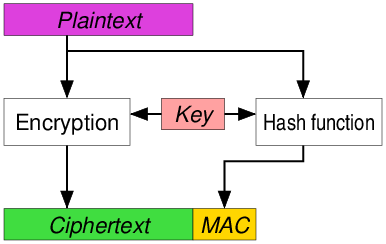
\includegraphics[width=\linewidth]{img/w4_applied_crypto_encrypt_and_mac.png}
 %\captionof{figure}{my caption of the figure}
\end{Figure}


\paragraph{MAC-then-encrypt}

\begin{myitemize}
     \item[$\xmark$] No integrity of ciphertext, need to decrypt (expensive)
     \item[$\checkmark$] Integrity of plaintext
     \item[$\checkmark$] No information about plaintext, MAC is encrypted
\end{myitemize}

\begin{Figure}
 \centering
 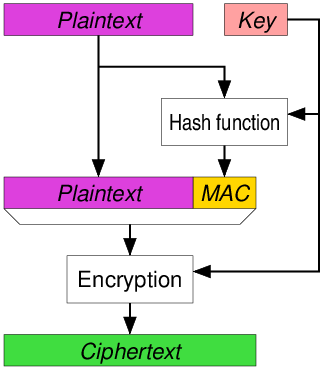
\includegraphics[width=\linewidth]{img/w4_applied_crypto_mac-then-encrypt.png}
\end{Figure}


\paragraph{Encrypt-then-MAC}


\begin{myitemize}
     \item[$\checkmark$] Integrity of ciphertext
     \item[$\checkmark$] Integrity of plaintext
     \item[$\checkmark$] No information leak, MAC encrypted
\end{myitemize}

\begin{Figure}
 \centering
 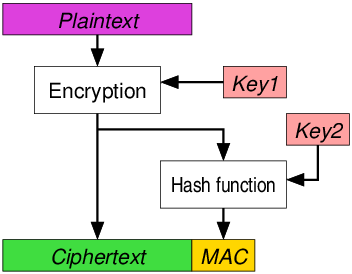
\includegraphics[width=\linewidth]{img/w4_applied_crypto_encrypt_then_mac.png}
\end{Figure}

\subsubsection{Authenticated Encryption with Associated Data (AEAD)}

\begin{myitemize}
     \item Combinations are easy to confuse 
     \item AEAD schemes provide authentication and confidentiality in one go
     \item Requires associated data, besides the key, message and nonce
     \item Output: ciphertext and tag
\end{myitemize}


\subsection{Asymmetric cryptography}

\begin{myitemize}
     \item Problems of symmetric crypto: how to securely share keys? How many keys such that everyone can talk to everyone?
     \item \textbf{Public key infrastructure}: public keys can be uploaded to public servers
     \item Integrity is obtained using \textbf{digital signatures}: a piece of data produced with private key and verifyable with public key
\end{myitemize}


\subsubsection{Digital signatures}

\begin{myitemize}
    \item Properties: integrity of message and authenticity of sender
    \item Non-repudiation (unlike MACs)
    \item Applications: Public key infrastructure and \textbf{certificates}
    \item An authority signs mapping between names and public keys, or names and verification keys
    \item Encryption key pair != signature key pair
\end{myitemize}

\subsubsection{Limitations}

\begin{myitemize}
    \item Computationally costly: compared to most symmetric key algorithms of equivalent security
    \item Slow
    \item Not suitable for large amounts of data
    \item Solution: \textbf{hybrid encryption}, sign hash of message and only encrypt small symmetric key
\end{myitemize}


\subsection{Hash functions}


\begin{myitemize}
    \item Only 1 input, no key
    \item Security properties:
    \begin{myitemize}
        \item Pre-image resistance: given H(m), difficult to get m
        \item Second pre-image resistance: given m, difficult to get an m'!=m such that H(m) = H(m'), m is fixed
        \item Collision resistance: difficult to find any m!=m' such that H(m) = H(m')
    \end{myitemize}
    \item Usage: \textbf{support digital signatures}, HMACs, password storage, file integrity, blockchain, ...
\end{myitemize}

\subsubsection{HMAC}

\begin{myitemize}
    \item H(K $||$ m) is \emph{not} a good HMAC, sensitive to length extension attacks (similar to those in CBC-MAC)
\end{myitemize}

\subsubsection{Digital signatures on hash functions}

\begin{myitemize}
    \item Sign the hash of the message h(m) instead of the message itself
    \item Second pre-image resistance: given signature of hash, cannot find another message with same hash (and thus same signature)
    \item Collision resistance: cannot sign a message and then claim they signed another message m'
\end{myitemize}

\subsubsection{Hybrid encryption}

\begin{myitemize}
    \item Asymmetric encryption is slow, symmetric is fast
    \item Use public keys: avoid sharing keys
    \item Use private key to encrypt actual data $\rightarrow$ \textbf{session key}
    \item Send/share private key with public-key encryption (small amount of data! fast)
    \item Still a problem! See forward secrecy
\end{myitemize}


\subsection{Diffie-Hellman key exchange}

\subsubsection{Forward secrecy}

\begin{myitemize}
    \item If at tome point in time, one of the two parties has its private key stolen, any past conversation might be decrypted (and future ones, if the private key is still used)
    \item Desirable property: forward secrecy, i.e. the secrecy of messages in a session is kept even if long term keys are compromised 
    \item Diffie-Hellman provides forward secrecy
\end{myitemize}

\subsubsection{Basic maths}

\begin{myitemize}
    \item Arithmetic modulo a number
    \item Arithmetic modulo a large prime p (> 1024 bits):
    \begin{myitemize}
        \item Addition and multiplication (mod p) can be computed
        \item Exponentiation $(a,x)\rightarrow a^x \mod p$ can be computed
        \item Discrete logarithms are hard, $(a, a^x\mod p) \rightarrow x=?$
    \end{myitemize}
\end{myitemize}

\subsubsection{Basic Diffie-Hellman key exchange}

\begin{myitemize}
    \item Shared public parameters p, g
    \item Both parties have random secret keys x, y
    \item Public keys $P_{Bob}=g^x \mod p$, $P_{Alice}=g^y\mod p$
    \item Shared session key (private!): $K=g^{xy}\mod p = (P_{Bob})^x = (P_{Alice})^y$
    \item After session is ended, delete secrets x and y. The session key can never be recovered, forward secrecy is achieved
\end{myitemize}


% ======================================= Authentication

\section{Authentication}

\begin{myitemize}
    \item Process of verifying a claimed identity
    \item NOT message authentication, in which the message comes from the designated sender and wasn't modified
    \item We saw authorization, i.e. whether a principal can access an asset, here we need to bind the user to a principal before authorization
    \item User or machine authentication
\end{myitemize}


\subsection{Ways to Prove Who You Are}

\begin{myitemize}
    \item Traditional: what you know, what you are, what you have
    \item Modern: where you are, how you act, who you know, ...
\end{myitemize}


\subsection{What you Know: Passwords}

\begin{myitemize}
    \item Password = shared secret between user and system
    \item Must consider many aspects!
    \item Secure transfer: eavesdropping \& impersonation, replay attacks, must secure the channel and use challenge-response protocols
    \item Secure storage: password database compromises, use pre-image resistant hash function, dictionnary attacks, parllel computing, rainbow tables $\rightarrow$ salt
    \item Secure checking: letter-by-letter checks induce timing leaks, consider typo flexibility?
    \item Secure passwords: put constraints, easy-to-remember pwds tend to be broken easily, often reused across different systems
    \item Use authentication libraries!!!
\end{myitemize}

\subsubsection{Challenge-Response Protocol - Password transfer}

Used to avoid replay attacks (for passwords and in general). For A that wants to login to B:

\begin{enumerate}
    \item A: I want to log in
    \item B: send a challenge: random number (from large space)
    \item A: encrypt password together with challenge
    \item Once B authenticated A, B deletes the challenge
\end{enumerate}

\subsubsection{Salted Hash - Password Storage}

\begin{myitemize}
    \item The only secure way to store passwords (no way do store in clear, hash alone not sufficient)
    \item Compute hash $h=H(pwd||salt)$ and store h alongside with the salt
    \item Less sensitive to dictionary attack: more computationally costly for the attacker
    \item Important: retrieving all passwords in a database is more difficult, but a targeted attack is equally difficult!
    \item Use slow hash functions
\end{myitemize}


\subsection{What you are - Biometrics}

\begin{itemize}
    \item Biometrics = measurement and statistical analysis of people's unique physical characteristics
    \item Examples: fingerprint, face recognition, retina, voice, handwritten signature, DNA
    \item Pros: nothing to remember, passive, difficult to delegate
    \item Two phases: enrolment and verification
\end{itemize}

\subsubsection{Enrolment}

\begin{myitemize}
     \item First phase of biometric authentication
     \item Introduction of the user biometric in the system and association with their login
     \item Capture of the biometric with the sensor $\rightarrow$ biometric template
\end{myitemize}

\subsubsection{Verification}

\begin{myitemize}
    \item Second phase of biometric authentication
    \item Capture and process biometric as before and compare biometric template with the stored one
    \item Local storage vs remote storage: local more privacy-preserving but harder to secure and update, remote is less-privacy-friendly but easy to secure and update
    \item Comparison is not exact: trade-off false positives and false negatives, depends on the context
\end{myitemize}

\subsubsection{Problems with Biometrics}

\begin{myitemize}
    \item Hard to keep secret: liveness detection
    \item Revocation is difficult/impossible
    \item Identifiable and unique: linking across systems
    \item May reveal private information: iris and disease, face and identity
    \item Not always immutable or universal: iris changes with lenses, fingerprint disappear
\end{myitemize}


\subsection{What you have: Tokens}

\begin{myitemize}
    \item Examples: smart card (signs a challenge sent by ATM to prove knowledge of a key), or device which output a number based on a secret and time (time syncronized with a server, number must match with server number)
    \item Step 1: offline initialization, common seed (random number) and clock syncronization
    \item Step 2: upon authentication request, both compute a number that depends on time, only a encrypted number is transferred by the token
    \item Note: the cryptographic function cannot be a hash since hashes do not require keys (everyone can compute it)
\end{myitemize}

\paragraph{Two Factor Authentication (2FA)}

\begin{myitemize}
    \item Combine two out of three factors: what you know, what you have, what you have
    \item Example: card = what you have + what you know (PIN)
    
\end{myitemize}

\subsection{Machine Authentication}

\begin{myitemize}
    \item Machines use public key cryptography to produce digital signatures
    \item Example: HTTPS/TLS to authenticate the server
    \item Defend from man in the middle $\rightarrow$ signatures
    \item Defend from replay attacks $\rightarrow$ challenges / nonces
\end{myitemize}


% =====================================================

\section{Adversarial thinking and attacks}

\subsection{Why Study Attacks?}

\begin{myitemize}
    \item Deeper understanding of defense: very good attackers make very good defenders, mediocre attackers make extremely poor defenders (asymmetry adversary-defender)
    \item Employability: penetration testing is a major industry
    \item Need both security and privacy
    \item Fail safe principle and sanitization: attack space cannot be completely explored (it's huge!), not finding an attack doesn't guarantee security
\end{myitemize}


\subsection{How are Attacks Deployed?}

\begin{myitemize}
    \item Attacks typically do not happen by chance
    \item Usually discovered by studying systems in systematic ways
\end{myitemize}

\subsubsection{The Security Engineering Process}

\begin{enumerate}
    \item Define security policy and threat model: what to protect from whom
    \item Define security mechanisms that support the policy given the threat model: how to protect it
    \item Build implementation that supports the mechanisms: implement protections
\end{enumerate}

\subsubsection{The Attack Engineering Process}

Inverse approach

\begin{enumerate}
    \item Exploit flaws in security policy and threat model: misidentified principals, assets, properties, capabilities beyond what considered in threat model (access, computational) = underestimation of the adversary
    \item Exploit flaws in security mechanisms: design weaknesses
    \item Exploit flaws in implementation: software is very complex, many small errors can enable adversary to infiltrate the TCB
\end{enumerate}


\subsection{Exploit flaws in security policy / threat model}

\paragraph{Exploiting misidentified assets in security policy}

\begin{myitemize}
    \item Example: Extract keys from Hardware Secure Modules (HSMs)
    \item HSM = CPU secured physically, hold crypto keys which can't be extracted by observing device (power consumption, computation timing, ...)
    \item Economy of mechanism: strict API, can access HSM through small set of functions
    \item HSMs implement PKCS\#11 standard for interoperability
    \item API to create a new key (internally!) from the secret key: given bit\_len and offset, uses bit\_len of the secret key from position offset
    \item Problem: PKCS\#11 considers the full key as an asset to protect, not the bytes of the key
    \item Procedure:
    \begin{enumerate}
        \item Ask  HSM to derive a new key of length 1 at offset 0
        \item Use new key to do an operation (e.g. HMAC) on known input
        \item Brute-force the key (input and output known, only 1 key byte)
        \item Repeat with keys at different offsets
    \end{enumerate}
\end{myitemize}


\paragraph{Exploiting unforeseen access capabilities}

\begin{myitemize}
    \item Example: from cable to the air. Engine Control Units (ECU) control the vehicle.  ECU connected to GSM/Wifi give a remote adversary access to the CAN bus and all the (safety) functions of the vehicle. Due to gradual evolution of technology (initially ECU not connected), this was lacking relevant security 
    \item Example: IoT devices are usually very poorly protected. Researchers at Princeton University showed that accessing those devices and changing their power consumption could crate arbitrary electricity demands (could bring down the grid). Much easier than getting in an electrical central!
    \item Example: Unilateral user authentication in GSM. When GSM was designed antennas were difficult and expensive to build. So operators did not implement authentication. But now, one can easily impersonate an antenna and make people connect to yours. 
\end{myitemize}


\paragraph{Exploiting unforeseen computational / algorithmic capabilities}

\begin{myitemize}
    \item Example (capabilities): NSA, brute-force against RSA keys
    \item Example (algorithmic side): machine learning revolution. Machine learning eases attacks: substitutes complex modeling tasks by data collection. 
    \item Note: machine learning also helps: improved malware detection, predicting zero days, identifying vulnerable devices, automated log analysis
\end{myitemize}


\subsection{Exploit flaws in security mechanisms}

\paragraph{Exploiting security mechanisms design weaknesses}

\begin{myitemize}
    \item Weak cryptographic primitives: Tesla (Key Fob algo) and A5/1 A5/2 for GSM
    \item Both examples used secret algorithms, security by obscurity is a bad idea, open design principle
\end{myitemize}


\subsection{Exploit flaws in implementation}

\paragraph{Exploiting bad operation decisions to subvert security mechanisms}
Example: WEP and bad use of RC4.  RC4 is a secure stream cipher. WEP used very small IV, so often repeated, and very bad

\paragraph{Exploiting implementation flaws to subvert security mechanisms}

Example: programmers make mistakes, besides bad parametrization of algorithms in implementations. Example of bug that allowed users to gain root access in Linux: wrong check in the implementation of the sudo command. 


\subsection{From specific to generic attacks}

\begin{myitemize}
    \item Ultimate goal: elevation of privilege or execution of arbitrary code in the TCB
    \item Specific attacks: problem in a particular security policy, threat model, mechanism. Adversary may violate a specific security property. 
    \item Generic attacks: get access to the TCB of the system, the adversary can violte all security properties
\end{myitemize}

\subsection{Reasoning about attacks}

\subsubsection{STRIDE}

\begin{myitemize}
    \item Helps security engineers to reason about threats to a system in a systematic way: what can go wrong?
    \item \textbf{S}poofing: authenticity
    \item \textbf{T}ampering: integrity
    \item \textbf{R}epudiation: non-repudiability
    \item \textbf{I}nformation disclosure: confidentiality
    \item \textbf{D}enial of service:  availability
    \item \textbf{E}levation of privilege: authorization
\end{myitemize}

\subsubsection{Common Weaknesses enumeration (CWE)}

\begin{myitemize}
    \item Idea: a database software errors leading to vulnerabilities to help security engineers avoid common pitfalls: what not to do. 
    \item MITRE has list of most dangerous software errors with consequences
\end{myitemize}

\paragraph{Insecure Interaction Between Components}

\begin{myitemize}
    \item One subsystem feeds another subsystem data that is \textbf{not sanitized}
    \item Class of errors: programmers do not check information that is sent between different components (non-sanitized)
    \item Example: OS Command Injection. Input controlled by adversary $\rightarrow$ command to the OS (POST HTTP method) 
    \item Example: Cross-site Scripting (XSS), improper neutralization of input during web page generation. Uses input to dynamically generate web content (GET HTTP method). 
    \item Avoid injection: sanitization! BIBA: never bring information from low (unknown) into high (OS, server). But very hard task: need to define the universe of good things
    \item Example: cross-site request forgery. Confused deputy (= browser) problem, enabled by ambient authority (= cookie-based authentication) 
    \item Avoid cross-site request forgery: don't accept cookies from unknown websites, use a challenge to avoid "reypling" cookies, don't use cookies
\end{myitemize}

\paragraph{Risky Resource Management}

\begin{myitemize}
    \item Software does not properly manage creation, usage, transfer, destruction of important system resources
    \item The system acts on non-sanitized input
    \item Example: family of buffer overflow bugs, mis-estimation of the space reserved in memory 
    \item TCB under the control of the adversary
\end{myitemize}

\paragraph{Porous defenses}

\begin{myitemize}
    \item Defensive techinques that are often misused, abused or just plain ignored
    \item Violation of complete mediation
    \item Failures and bugs in authentication, authorization, encryption
    \item 
\end{myitemize}

\begin{myitemize}
    \item 
\end{myitemize}

\begin{myitemize}
     \item[$o$] f
\end{myitemize}


\end{multicols}
\end{document}
